% Ubah kalimat sesuai dengan judul dari bab ini
\chapter{PROFIL PERUSAHAAN}

% Ubah konten-konten berikut sesuai dengan yang ingin diisi pada bab ini

\section{Program Google Bangkit}

  % Contoh input gambar dengan format *.png
\begin{figure} [ht] \centering
  % Nama dari file gambar yang diinputkan
  
\includegraphics[scale=0.7]{gambar/bangkit.jpg}
  % Keterangan gambar yang diinputkan
  \caption{Google Bangkit \cite{logo}}
  % Label referensi dari gambar yang diinputkan
  \label{fig:OrganizationStructure}
\end{figure}

Program Google Bangkit \cite{bangkit} merupakan program pengembangan kemampuan mahasiswa di bidang teknologi yang dicetuskan dalam kerjasama antara Dirjen Pendidikan Tinggi Kemendikbud, Google, Gojek, Tokopedia, Traveloka, dan mitra perguruan tinggi.
Program ini ditawarkan melalui program Kampus Merdeka untuk 3000 mahasiswa yang berhasil lolos melawati serangkaian tes seleksi.

Pada tahun 2020, program Google Bangkit hanya meliputi kurikulum \textit{machine learning} di mana pada tahun 2021 berubah menjadi \textit{machine learning}, \textit{cloud computing}, dan \textit{mobile development}.
Di setiap jalur pembelajaran, peserta juga akan mempelajari keterampilan penting yang berguna untuk pengembangan karir di masa depan, seperti contoh:

  \begin{enumerate}[nolistsep]
    
    \item \textit{Design Thinking}
    
    \item \textit{Leadership}
    
    \item \textit{Communication}
    
    \item \textit{Entrepreneurship}
    
    \item \textit{Presentation Skills}
  
  \end{enumerate}

Bangkit mendapat antusias yang luar biasa, hampir 28.000 pendaftar dari 500 perguruan tinggi di seluruh Indonesia.
Kemudian mereka mengikuti proses aplikasi dan seleksi yang komprehensif, 3000 mahasiswa lolos seleksi dan diundang untuk mendaftar.
Dari mereka yang mendaftar, 30\% adalah perempuan dan sekitar 29\% diantaranya berasal dari latar belakang non-CS/IT.
Program Bangkit bekerja sama dengan 15 universitas mitra dan mahasiswa terpilih akan mengikuti pengalaman belajar online di Google Bangkit selama 18 minggu mulai Februari 2021.
Para mahasiswa akan didampingi oleh \textit{coach}/mentor dari industri dan perguruan tinggi.
Di akhir semester, akan dipilih lima belas tim proyek akhir untuk pengembangan lebih lanjut termasuk hibah inkubasi dan dukungan dari perguruan tinggi mitra Bangkit.
Peserta yang menyelesaikan program ini mendapatkan hingga 20 sks (satuan kredit semester) dari perguruan tingginya (tergantung persetujuan universitas peserta).

\section{Visi dan Misi}

Program Google Bangkit memiliki visi misi untuk mempersiapkan siswa dengan keterampilan yang dibutuhkan dan sertifikasi teknologi.
Program ini menyediakan fasilitas pengajaran di tiga bidang yang berbeda, yaitu \textit{machine learning}, \textit{cloud computing}, dan \textit{mobile development}.
Materi yang dihadirkan di dalam program ini berasal dari kursus daring yang disediakan oleh \textit{MOOC} terkenal dan berkualitas, serta mendapatkan pengajaran langsung dari praktisi-praktisi industri \textit{startup} terkemuka Indonesia maupun luar Indonesia.
Pada akhir program ini, peserta akan dilengkapi dengan keahlian teknologi dan \textit{soft skill} yang dibutuhkan untuk berpindah dari dunia akademis ke tempat kerja dan sukses di perusahaan terkemuka \cite{logo}.

\section{Struktur Organisasi}

Struktur Organisasi dari program Google Bangkit cukup sederhana.

% Contoh input gambar dengan format *.png
\begin{figure}[ht] \centering
  % Nama dari file gambar yang diinputkan
  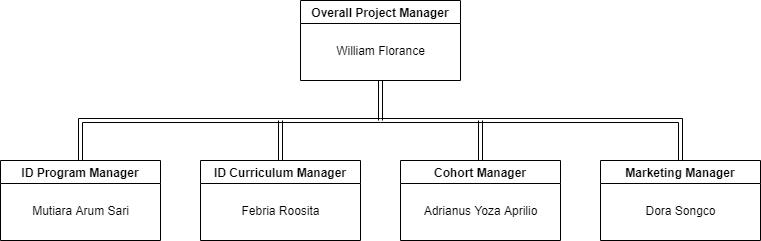
\includegraphics[scale=0.4]{gambar/struktur-organisasi.png}
  % Keterangan gambar yang diinputkan
  \caption{Struktur Organisasi Program Bangkit}
  % Label referensi dari gambar yang diinputkan
  \label{fig:strukturOrg}
\end{figure}

% Contoh penggunaan referensi dari gambar yang diinputkan
Seperti yang bisa dilihat pada gambar \ref{fig:strukturOrg}, dapat diketahui bahwa program ini dipimpin oleh William Florance sebagai \textit{Overall Prject Manager}, Mutiara Arum Sari sebagai \textit{ID Program Manager}, Febria Roosita sebagai \textit{ID Curriculum Manager}, Adrianus Yoza Aprilio sebagai \textit{Cohort Manager}, dan Dora Songco sebagai \textit{Marketing Manager}